\documentclass[10pt]{article}

\usepackage[mode=buildnew,subpreambles=true]{standalone}
%%%% PACKAGES

\usepackage{import}
\usepackage[toc,page]{appendix}
\usepackage[T1]{fontenc}
\usepackage[english]{babel}
\usepackage[utf8]{inputenc}
\usepackage{graphicx}
\usepackage{adjmulticol}
\usepackage[labelfont=bf]{caption}
\usepackage{float}
\usepackage{graphicx}
\usepackage{subcaption}
\usepackage{fancyhdr}
\usepackage{url}
\usepackage{amsmath} % collection de symboles mathématiques
\usepackage{amssymb} % collection de symboles mathématiques
\usepackage{amsthm}
\usepackage{bbm}
\usepackage{bm}
\usepackage{stmaryrd}
\usepackage{mathtools}
\usepackage{cancel}
\usepackage{titling}
\usepackage{nameref} % pour désigner des parties par leur nom
\usepackage{url} % pour mettre des URL
\usepackage{cite}
% \usepackage[sectionbib]{chapterbib}
% \usepackage{chapterbib}
\usepackage[numbers,sort&compress]{natbib}
% \usepackage[square,numbers,sectionbib]{natbib}
% \usepackage{bibunits}
% \usepackage{biblatex}
\usepackage{tabularx}
\usepackage{titlesec, blindtext, color}
% \usepackage{auto-pst-pdf}

%%%% TIKZ

\usepackage{pgf, tikz}
\usetikzlibrary{shapes.misc}
\usetikzlibrary{decorations.pathreplacing}

\tikzset{cross/.style={cross out, draw=black, minimum size=2*(#1-\pgflinewidth), inner sep=0pt, outer sep=0pt},
%default radius will be 1pt.
cross/.default={0.25pt},
    point/.style={
    thick,
    draw=black,
    cross out,
    inner sep=0pt,
    minimum width=4pt,
    minimum height=4pt,
    },
}

%%%% STYLE

\textheight=25 true cm
\textwidth= 20. true cm
\oddsidemargin=-1.75truecm
\evensidemargin=0.5truecm
\topmargin=-3 truecm

% \setlength{\topmargin}{-1cm}
% \setlength{\headheight}{0.43cm}
% \setlength{\headsep}{0.8cm}
% \setlength{\footskip}{0cm}
% \setlength{\textwidth}{17cm}
% \setlength{\textheight}{23.5cm}
% \setlength{\voffset}{-2.5cm}
% \setlength{\hoffset}{-0.25cm}
% \setlength{\oddsidemargin}{0cm}
% \setlength{\evensidemargin}{0cm}
\setlength{\parindent}{0pt}
\setlength{\footskip}{1.5cm}

\setlength{\droptitle}{-1cm}

\setcounter{tocdepth}{3}
\setcounter{secnumdepth}{3}

\definecolor{lcolor}{rgb}{0,0,0.6} % définition de la couleur des liens pdf
\usepackage{hyperref}
\hypersetup{pdftex,colorlinks=true,
linkcolor=lcolor,
citecolor=lcolor,
urlcolor=lcolor,
hyperindex=true,
hyperfigures=false} % fichiers pdf 'intelligents', avec des liens entre les références, etc.

\definecolor{gray75}{gray}{0.75}

\AtBeginDocument{\addtocontents{toc}{\protect\thispagestyle{empty}}}

% \titleformat{\chapter}[hang]{\vspace{-50pt}\huge\bfseries}{\thechapter\hspace{20pt}\textcolor{gray75}{|}\hspace{20pt}}{0pt}{\huge\bfseries}
\titleformat{\subsection}[block]{\hspace{0em}}{\large\textbf\thesubsection}{1em}{\large\textbf}
\titleformat{\subsubsection}[block]{\hspace{0em}}{\Small\textbf\thesubsubsection}{1em}{\Small\textbf}

\usepackage{etoolbox}
\makeatletter
\patchcmd{\@chap@pppage}{\thispagestyle{plain}}{\thispagestyle{empty}}{}{}
\makeatother

\captionsetup{font=normalsize}
\captionsetup[sub]{font=scriptsize}

%%%% COMMANDS

\providecommand{\ie}{\textit{i.e.}~}

%\renewcommand*\thesection{\arabic{section}}

\makeatletter
\providecommand*\bigcdot{\mathpalette\bigcdot@{.5}}
\providecommand*\bigcdot@[2]{\mathbin{\vcenter{\hbox{\scalebox{#2}{$\m@th#1\bullet$}}}}}
\makeatother

\providecommand{\appropto}{\mathrel{\vcenter{
  \offinterlineskip\halign{\hfil$##$\cr
    \propto\cr\noalign{\kern2pt}\sim\cr\noalign{\kern-2pt}}}}}

\providecommand\encircle[1]{%
  \tikz[baseline=(X.base)]
    \node (X) [draw, shape=circle, inner sep=0] {\strut #1};}

\providecommand\phantomarrow[2]{%
  \setbox0=\hbox{$\displaystyle #1\to$}%
  \hbox to \wd0{%
    $#2\mapstochar
     \cleaders\hbox{$\mkern-1mu\relbar\mkern-3mu$}\hfill
     \mkern-7mu\rightarrow$}%
  \,}

\providecommand{\myparagraph}[1]{\paragraph{#1}\mbox{}\\\vspace{-5pt}}

\providecommand{\isEquivTo}[1]{\underset{#1}{\sim}}

\makeatletter
\providecommand{\subalign}[1]{%
  \vcenter{%
    \Let@ \restore@math@cr \default@tag
    \baselineskip\fontdimen10 \scriptfont\tw@
    \advance\baselineskip\fontdimen12 \scriptfont\tw@
    \lineskip\thr@@\fontdimen8 \scriptfont\thr@@
    \lineskiplimit\lineskip
    \ialign{\hfil$\m@th\scriptstyle##$&$\m@th\scriptstyle{}##$\crcr
      #1\crcr
    }%
  }
}
\makeatother

% \makeatletter
% % Original \l@section:
% %\renewcommand*\l@section{\vskip 6pt plus 1pt minus 1pt
% %                         \@dottedtocline{1}{1.5em}{2.3em}}
% % Modified \l@section:
% \renewcommand*\l@section{\ifnum\c@tocdepth>\z@\vskip 6pt plus 1pt minus 1pt \fi
%                          \@dottedtocline{1}{1.5em}{2.3em}}
% \makeatother

\providecommand\smallO[1]{
      \mathchoice
         {% mode \displaystyle
            \ensuremath{\mathop{}\mathopen{}{\scriptstyle\mathcal{O}}\mathopen{}\left(#1\right)}
         }
         {% mode \textstyle
            \ensuremath{\mathop{}\mathopen{}{\scriptstyle\mathcal{O}}\mathopen{}\left(#1\right)}
         }
         {% mode \scriptstyle
            \ensuremath{\mathop{}\mathopen{}{\scriptscriptstyle\mathcal{O}}\mathopen{}\left(#1\right)}
         }
         {% mode \scriptscriptstyle
            \ensuremath{\mathop{}\mathopen{}{o}\mathopen{}\left(#1\right)}
         }
   }

%%%% PATCH

% \makeatletter
% \let\orig@document\document
% \let\orig@enddocument\enddocument
% \def\sa@document{%
%   \endgroup
%   \global\let\enddocument\sa@enddocument
%   \sa@atbegindocument
% }
% \def\sa@enddocument{%
%   \sa@atenddocument
%   \global\let\document\orig@document
%   \global\let\enddocument\orig@enddocument
%   \begingroup
%   \@ignoretrue
%   \def\@currenvir{document}%
%   \aftergroup\endinput
% }
% \makeatother


\title{\bf Error in the cloning algorithm}
\author{Yann-Edwin Keta}
\date{January 5th, 2019}

\begin{document}

\maketitle

We consider the following modified equation of rotational motion,
\begin{equation}
\dot{\theta}_i = - g \, N \, \frac{\partial}{\partial \theta_i} |\underline{\nu}(t)|^2 + \sqrt{\frac{2}{\alpha \, \text{Pe}}} \xi_i,
\end{equation}
with $g$ a free parameter.\\

According to notes by Takahiro, summarised in \href{https://yketa.github.io/DAMTP_2019_Wiki/#ABP%20cloning%20algorithm}{this tiddler}, we should have that
\begin{equation}
\left. s \, w_{\text{mod}}(0, \tau) \right|_{s=0} =  \frac{1}{N} - \underbrace{\frac{1}{\tau} \int_0^{\tau} |\underline{\nu}(t)|^2 \, \text{d}t}_{\mathcal{I}_1(0, \tau)} - g^2 \, \alpha \, \text{Pe} \, \underbrace{\frac{1}{N \, \tau} \int_0^{\tau} |\underline{\nu}(t)|^2 \, \sum_{i=1}^N \sin^2(\theta_i(t) - \varphi(t)) \, \text{d}t}_{\mathcal{I}_2(0, \tau)},
\label{swmod}
\end{equation}
with
\begin{equation}
\lim_{\tau \rightarrow \infty} \mathcal{I}_1(0, \tau) = \left<|\underline{\nu}(t)|^2\right>_{\text{mod}} = \frac{1}{N}\frac{1}{1 + g \, \alpha \, \text{Pe}},
\label{I1}
\end{equation}
which we check in figure \ref{testI1}.

\begin{figure}[H]
\centering
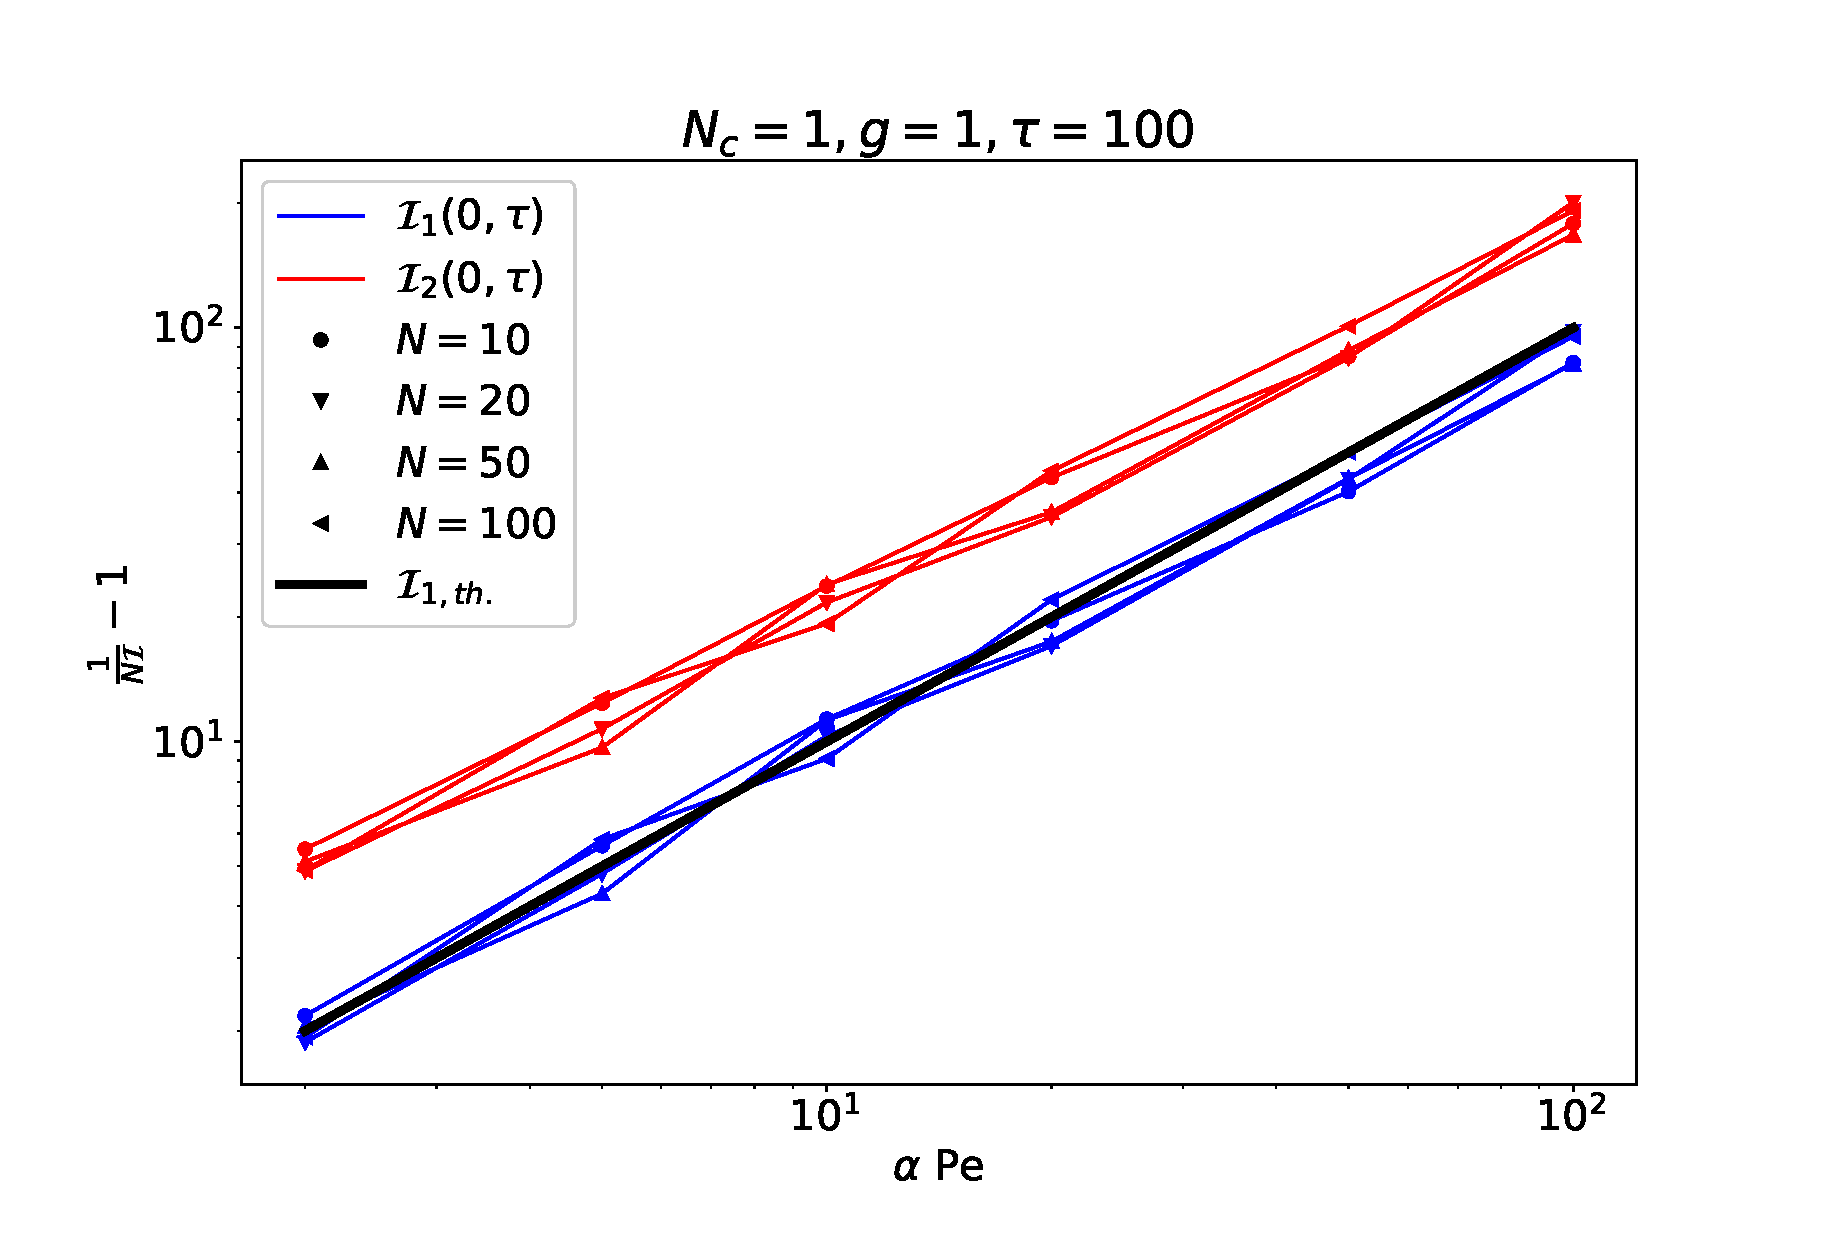
\includegraphics[width=0.65\textwidth]{testI1.eps}
\caption{Output from our cloning algorithm.}
\label{testI1}
\end{figure}

Considering a single clone, $N_c = 1$, we approximate the scaled cumulant generating function with
\begin{equation}
\psi(s=0, \tau) = \left. - s \, w_{\text{mod}}(0, \tau)\right|_{s=0},
\end{equation}
and we note that
\begin{equation}
\psi(s=0, \tau) = \left.\frac{1}{N \, \tau} \log\left<e^{-s \, N \, \tau \, w(0, \tau)}\right>_0\right|_{s=0} = 0,
\end{equation}
which with equations \ref{swmod} and \ref{I1} should lead to
\begin{equation}
\left. \mathcal{I}_2(0, \tau) \right|_{s=0} = \frac{1}{N} \frac{1}{g + g^2 \, \alpha \, \text{Pe}},
\end{equation}
and in particular, for $g = 1$, to
\begin{equation}
\left. \mathcal{I}_2(0, \tau) \right|_{s=0, g=1} = \left. \mathcal{I}_1(0, \tau) \right|_{s=0, g=1},
\end{equation}
which we see from figure \ref{testI1} is not satisfied.\\

We can see this discrepancy from the fact that
\begin{equation}
0 \leq \frac{1}{N} \sum_{i=1}^N \sin^2(\theta_i(t) - \varphi(t)) \leq 1,
\end{equation}
and thus
\begin{equation}
\mathcal{I}_2(0, \tau) \leq \mathcal{I}_1(0, \tau).
\end{equation}
Moreover, we have that the unbiased dynamics, $s = 0$, should not display orientational order, $|\underline{\nu}(t)| \approx 0$ for $N \rightarrow \infty$. Heuristically, considering that the $\theta_i$ are randomly distributed, we should get that
\begin{equation}
\left<\frac{1}{N} \sum_{i=1}^N \sin^2(\theta_i(t) - \varphi(t)) \right> \approx \left<\sin^2\right> = \frac{1}{2},
\end{equation}
which may explain the approximate relation
\begin{equation}
\mathcal{I}_2(0, \tau) \approx \frac{1}{2} \mathcal{I}_1(0, \tau),
\end{equation}
we observe numerically.

\end{document}
